\chapter{Wyniki}
\label{cha:wyniki}

W tym rozdziale opisana jest metodologia testowania wydajności algorytmów mnożenia macierzy rzadkiej z wektorem dla wartości pojedynczej precyzji (\textit{SpMV}) oraz dokonana jest analiza uzyskanych wyników.

System wykorzystany do przeprowadzenia testów wydajności wyposażony był w procesor graficzny NVIDIA RTX 3060 (GA106) w konfiguracji 130W, działający pod sterownikiem w wersji 528.24.
Systemem operacyjnym był Windows 11 w wersji 22H2, kompilator \textit{glslc} \cite{glslcgithub} w wersji v2021.2 oraz VulkanSDK \cite{vulkansdk} w wersji 1.2.182.0.
Na potrzeby testów wykorzystano pięć macierzy: BEAFLW, DENSE2, BCSSTK32, SCIRCUIT i GA41AS41H72.
Każda z nich reprezentuje różne cechy macierzy rzadkich: rozmiar, zagęszczenie, rozpiętość wartości w komórkach i sposób rozmieszczenia elementów.
Każdy algorytm dla danego formatu uruchamiany był 1000 razy, celem zdobycia średniego czasu wykonania danej operacji.

\begin{figure}[!htb]
\minipage{0.45\textwidth}
    \textbf{BEAFLW} ma wymiar $497 \times 507$, z czego $21.193\%$ jest elementami niezerowymi, rozkład przestawiony na rysunku \ref{beaflw_matrix_plot} wykazuje znikome skumulowanie względem przekątnej.
\endminipage\hfill
\minipage{0.45\textwidth}
  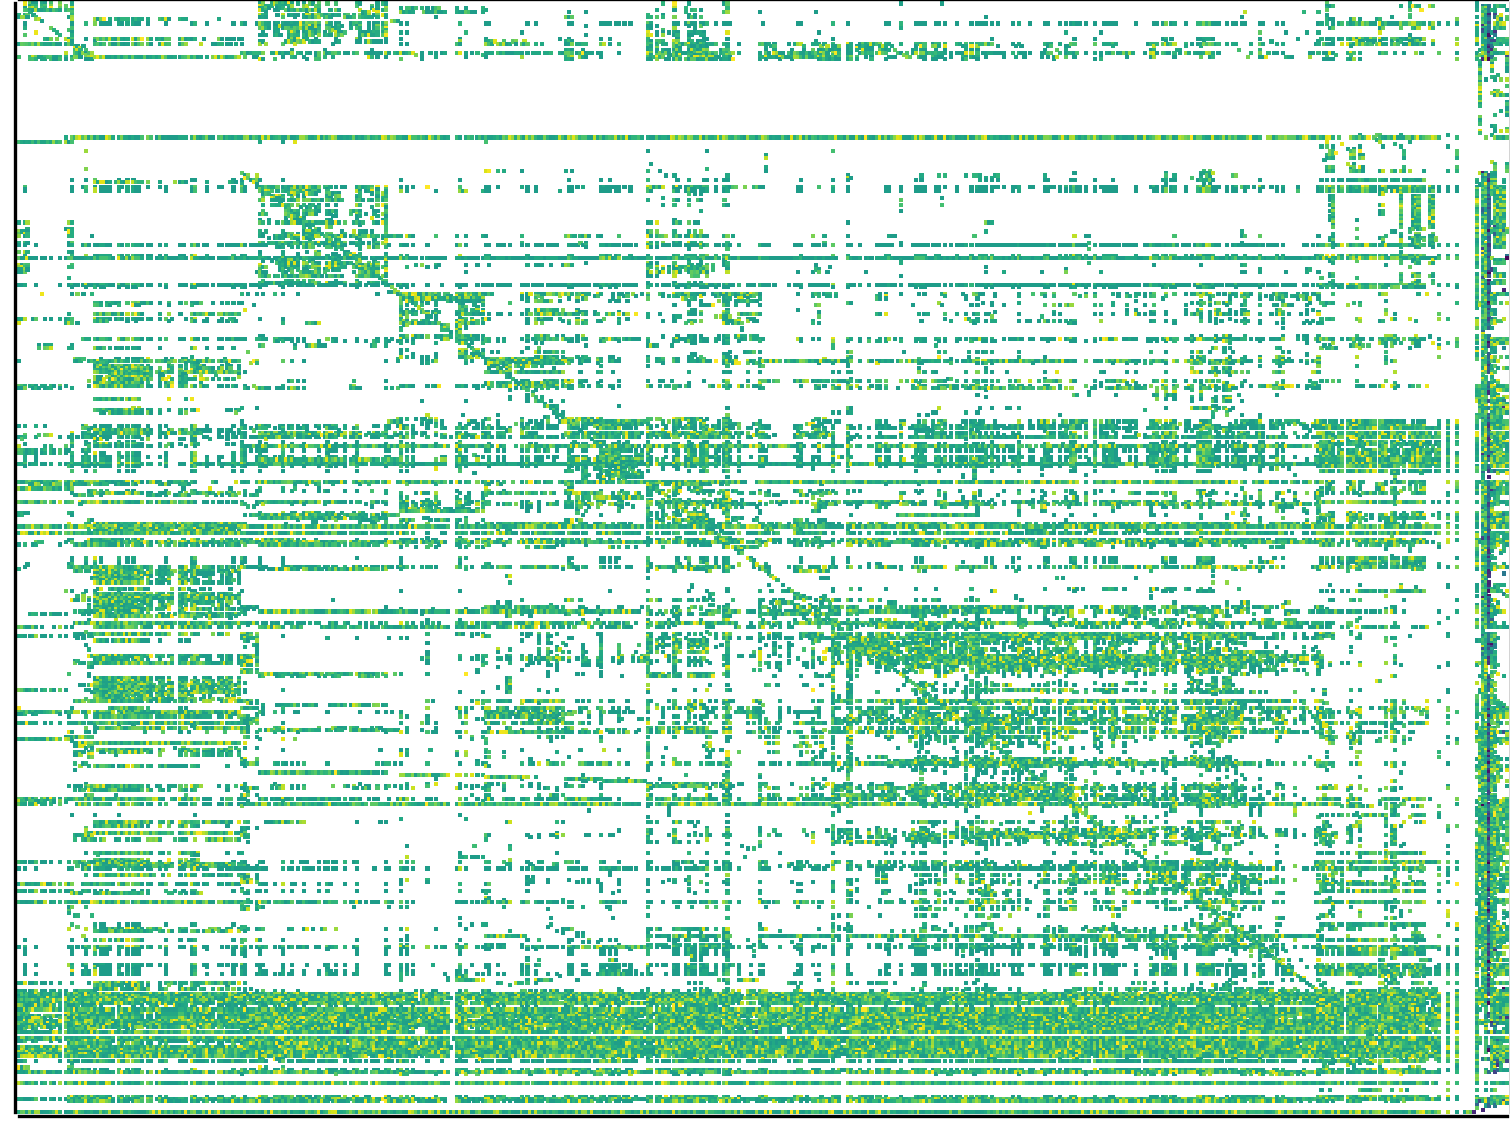
\includegraphics[width=\linewidth]{matrix_plots/beaflw.png}
  \caption{Rozkład w macierzy BEAFLW}\label{beaflw_matrix_plot}
\endminipage\hfill
\end{figure}

\pagebreak

\begin{figure}[!htb]
\minipage{0.45\textwidth}
    \textbf{DENSE2} ma wymiar $2000 \times 2000$, z czego $100\%$ elementów ma wartości niezerowe, rozkład przestawiony na rysunku \ref{dense2_plot}.
\endminipage\hfill
\minipage{0.45\textwidth}
  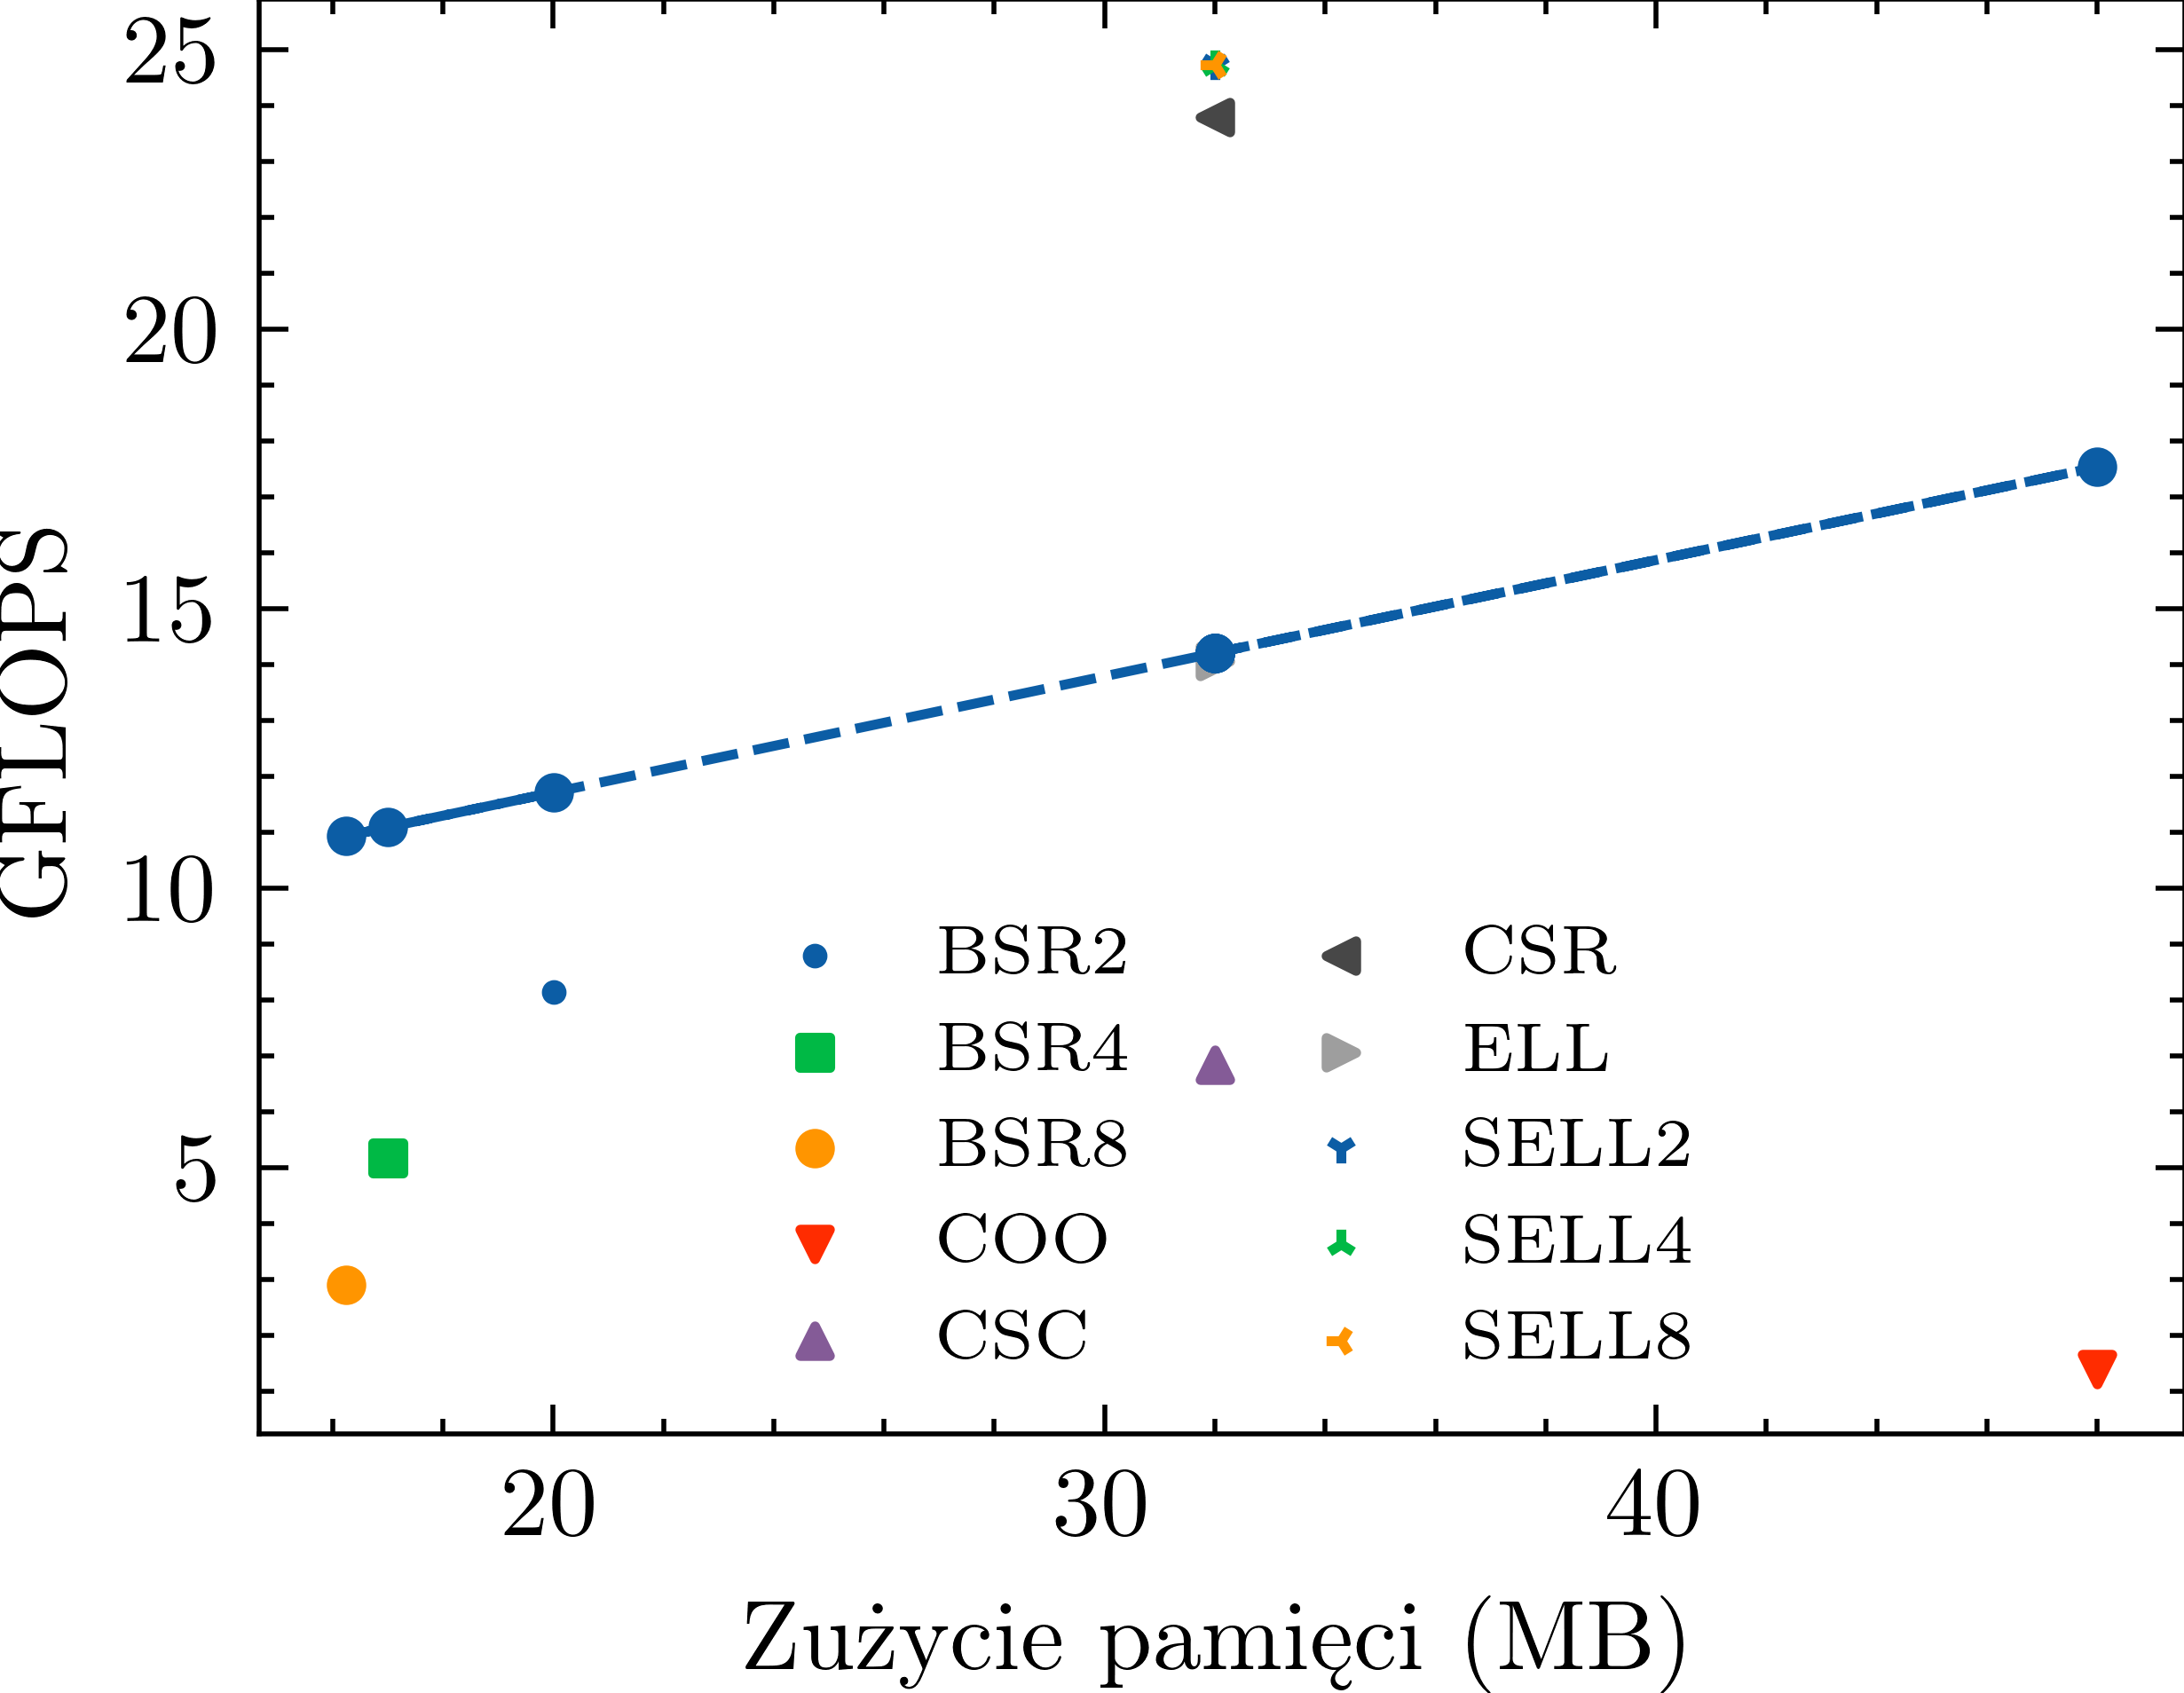
\includegraphics[width=\linewidth]{matrix_plots/dense2.png}
  \caption{Rozkład w macierzy DENSE2}\label{dense2_plot}
\endminipage\hfill
\end{figure}

\begin{figure}[!htb]
\minipage{0.45\textwidth}
    \textbf{BCSSTK32} ma wymiar $44609 \times 44609$, z czego $0.1\%$ jest elementami niezerowymi, rozkład przestawiony na rysunku \ref{bcsstk32_plot} wykazuje symetryczność względem przekątnej i niskie skumulowanie względem niej.
\endminipage\hfill
\minipage{0.45\textwidth}
  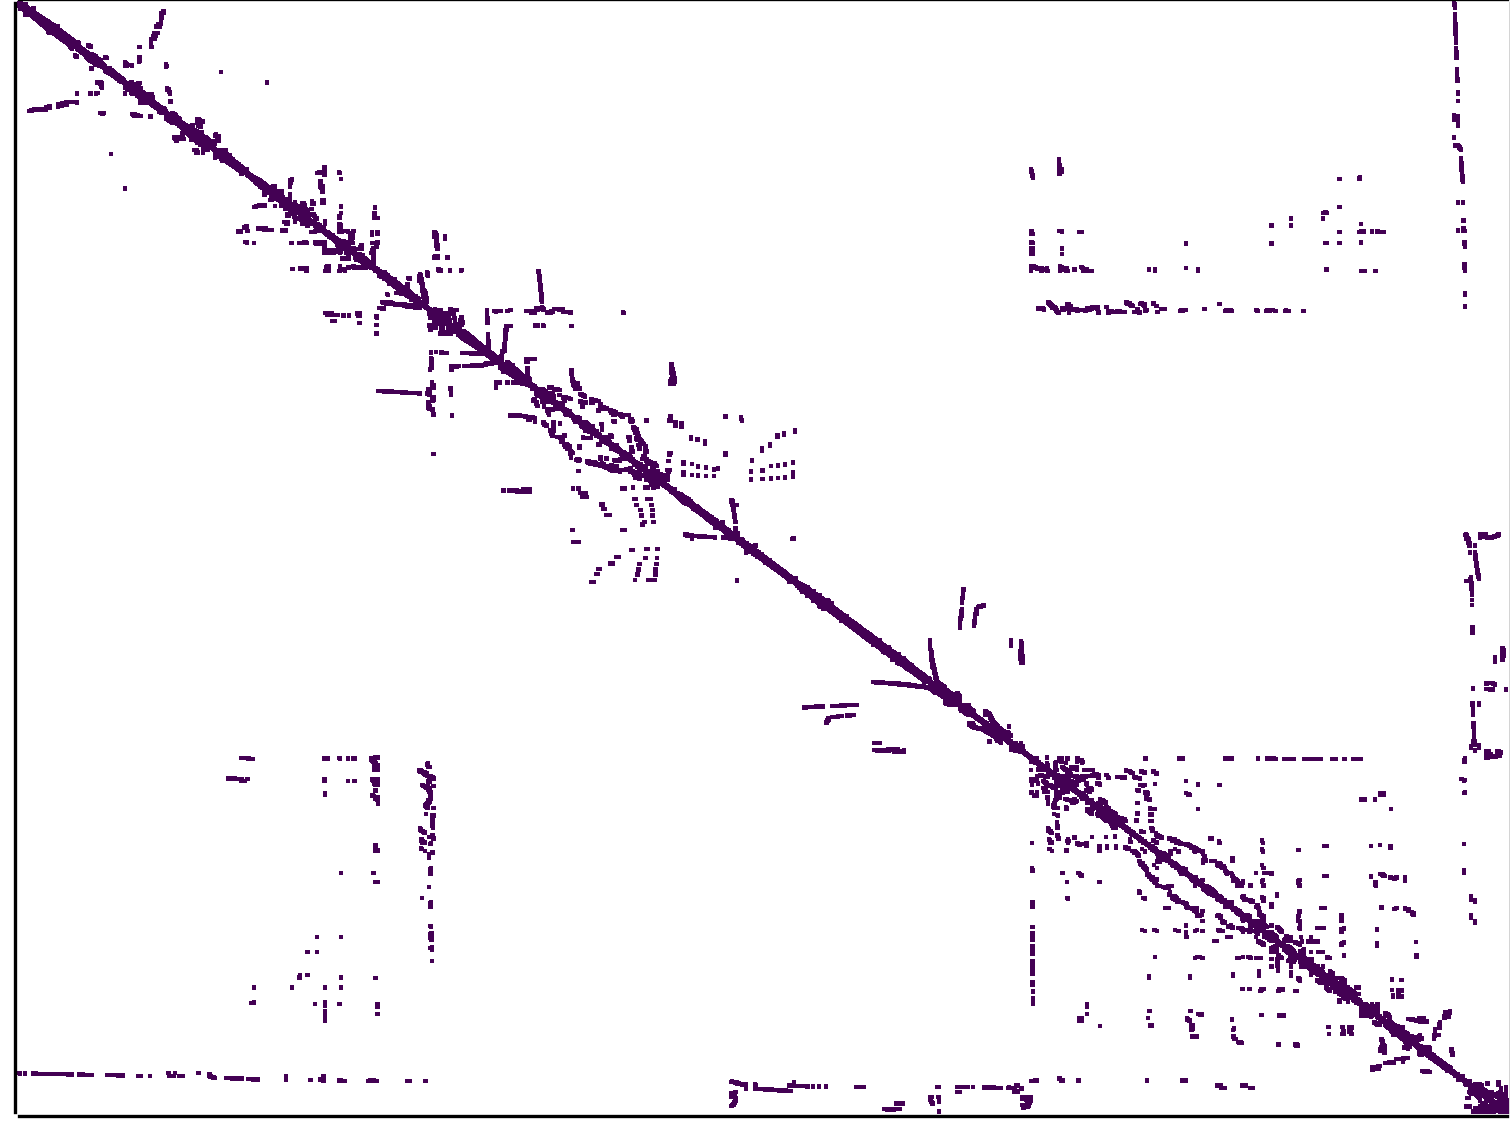
\includegraphics[width=\linewidth]{matrix_plots/bcsstk32.png}
  \caption{Rozkład w macierzy BCSSTK32}\label{bcsstk32_plot}
\endminipage\hfill
\end{figure}

\begin{figure}[!htb]
\minipage{0.45\textwidth}
    \textbf{SCIRCUIT} ma wymiar $170998 \times 170998$, z czego $0.003\%$ jest elementami niezerowymi, rozkład przestawiony na rysunku \ref{scircuit_plot} wykazuje symetryczność względem przekątnej i średnie skumulowanie względem niej.
\endminipage\hfill
\minipage{0.45\textwidth}
  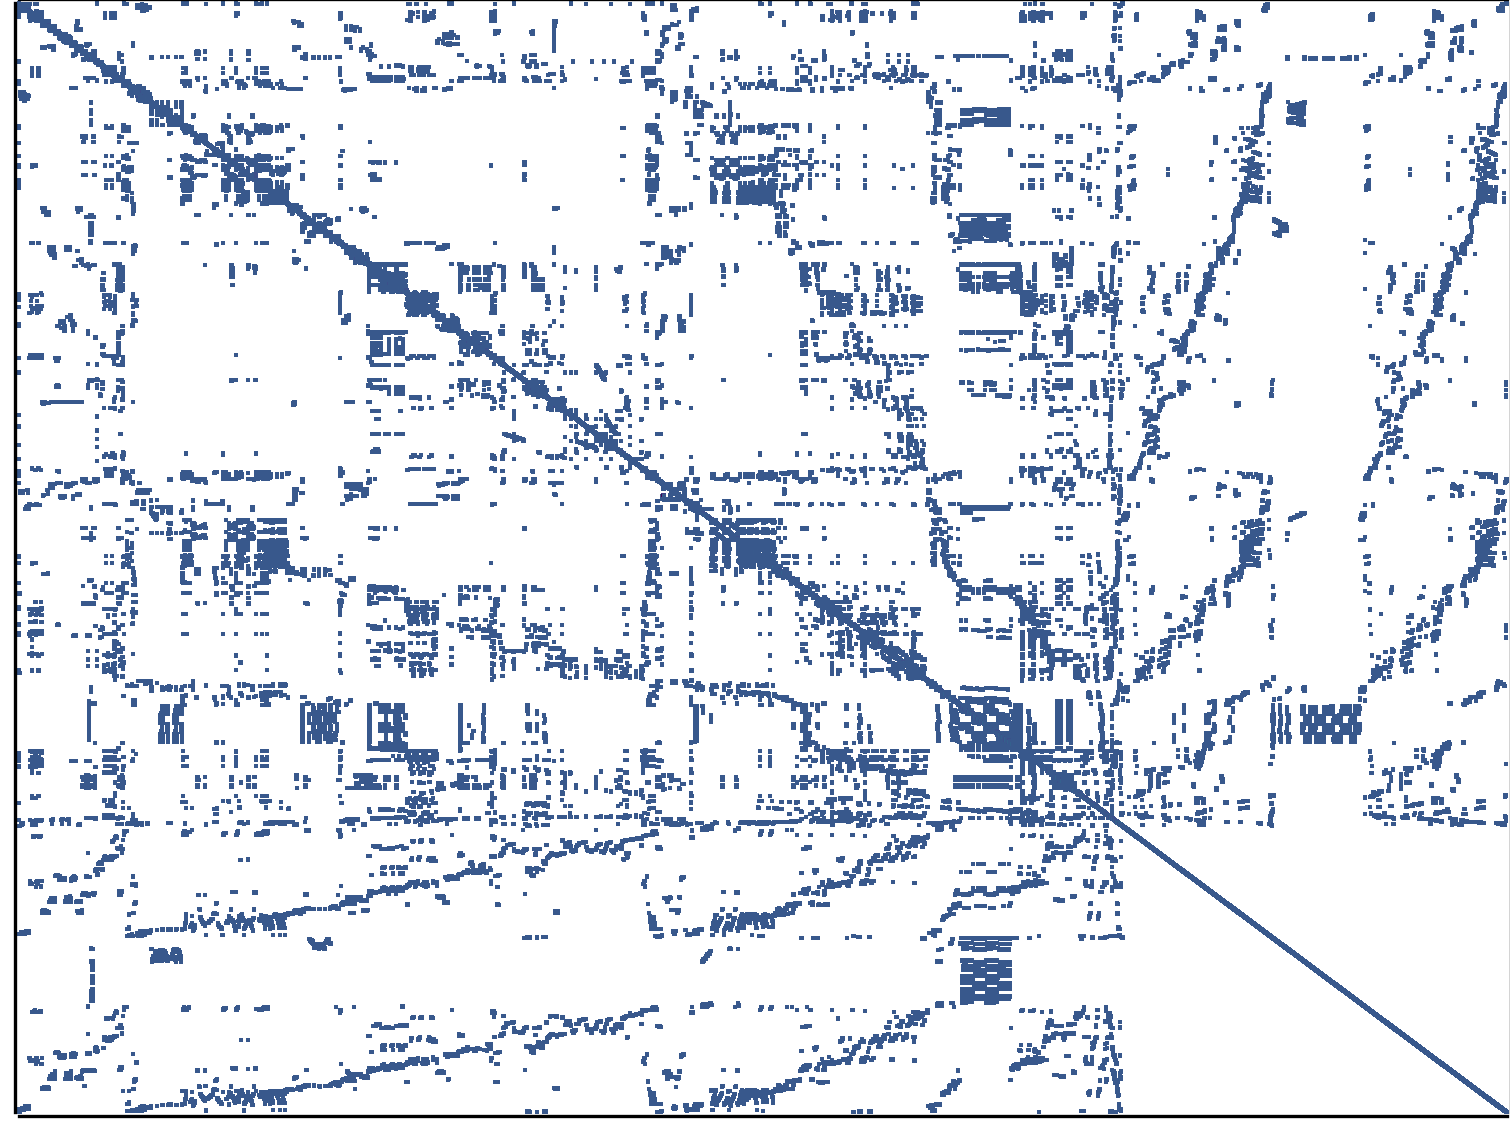
\includegraphics[width=\linewidth]{matrix_plots/scircuit.png}
  \caption{Rozkład w macierzy SCIRCUIT}\label{scircuit_plot}
\endminipage\hfill
\end{figure}

\pagebreak

\begin{figure}[!htb]
\minipage{0.45\textwidth}
    \textbf{GA41AS41H72} ma wymiar $268096 \times 268096$, z czego $0.026\%$ jest elementami niezerowymi, rozkład przestawiony na rysunku \ref{ga41as41h72_plot} wykazuje symetryczność względem przekątnej i wysokie skumulowanie względem niej.
\endminipage\hfill
\minipage{0.45\textwidth}
  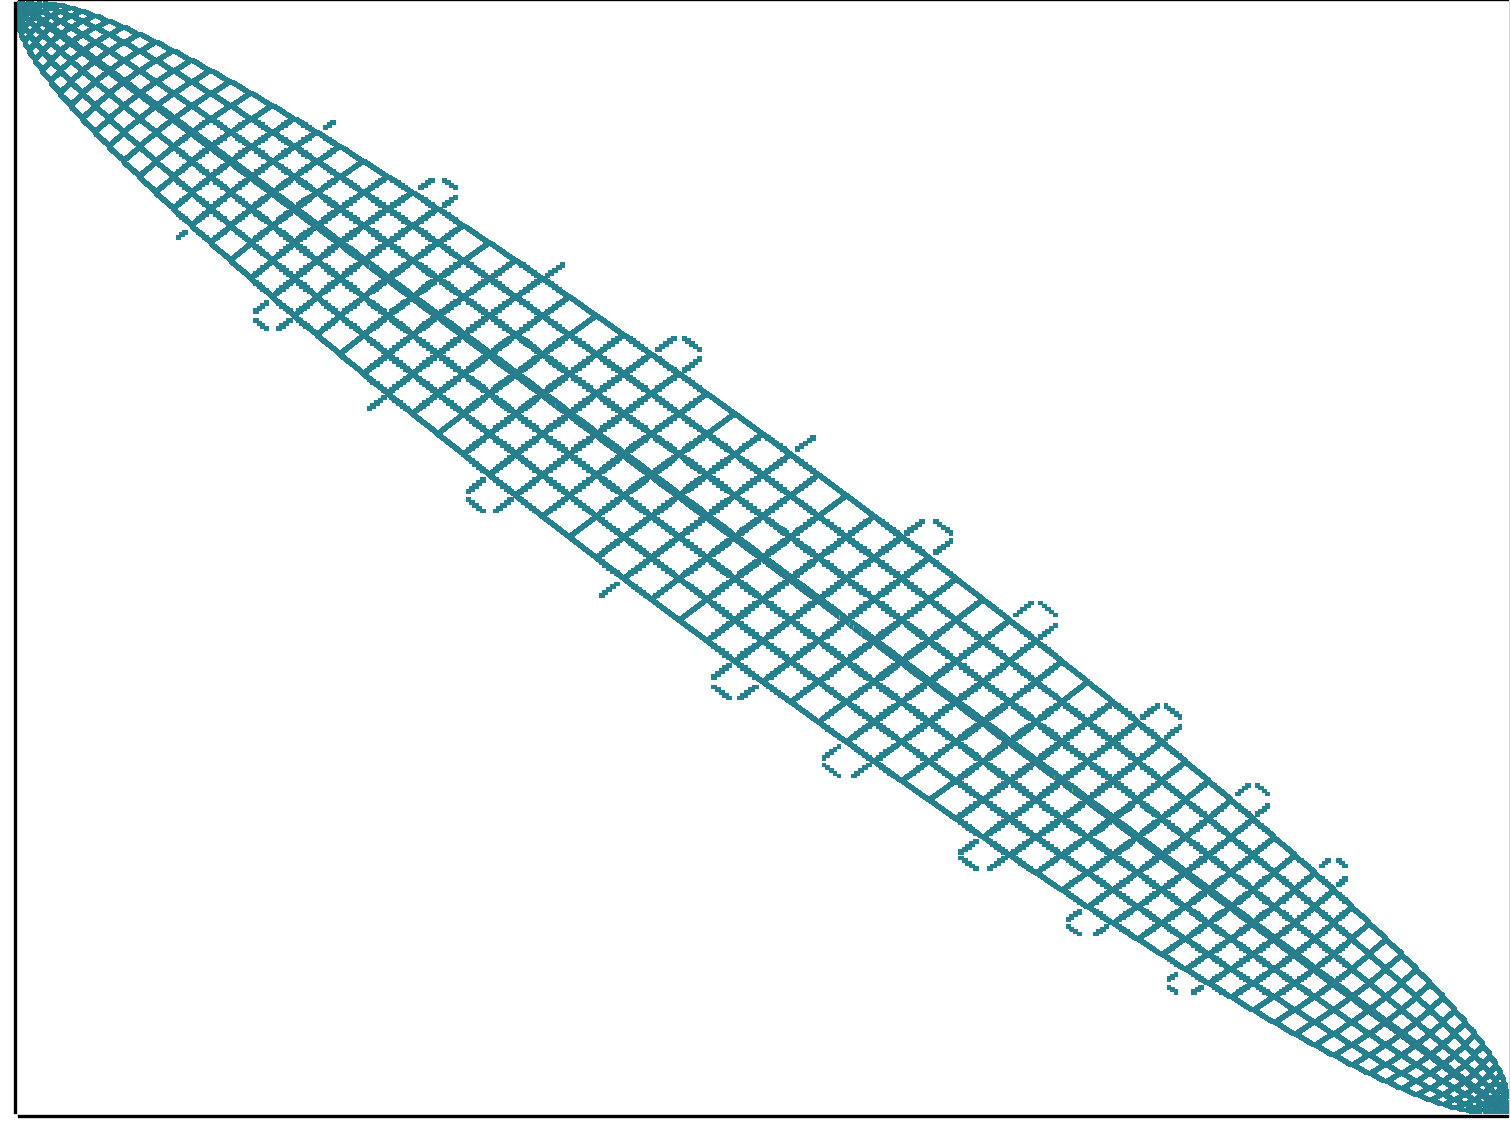
\includegraphics[width=\linewidth]{matrix_plots/Ga41As41H72.png}
  \caption{Rozkład w macierzy GA41AS41H72}\label{ga41as41h72_plot}
\endminipage\hfill
\end{figure}

Analizując wykres \ref{all_plot} zauważalna jest wysoka wydajność formatu CSR. W dwóch przypadkach jest najwyższa, natomiast w pozostałych jest blisko największej osiągniętej wydajności. 
Format SELL wraz ze wzrostem $C$ osiąga wyższe wyniki, w niektórych przypadkach będąc bardziej wydajnym niż CSR, natomiast dla niektórych macierzy, gdy $C$ stawało się większe niż $4$ wydajność spadała.
Wydajność formatu ELL nie wyróżniała się ponad inne formaty, pomimo znacznie większego zużycia pamięci.
W ponad połowie przypadków format ten był szybszy niż COO i CSC, natomiast dla macierzy z małym zagęszczeniem lub małą ilością elementów format COO osiągał najwyższą wydajność ze wszystkich formatów.
Pomimo najmniejszego zużycia pamięci format BSR osiągał wyniki zawsze gorsze od SELL i CSR, nawet dla macierzy DENSE2, która idealnie wypełnia całą macierz blokami bez elementów zerowych, poza tą macierzą wraz ze wzrostem rozmiaru bloku wydajność spadała.

\begin{figure}[!htb]
    \centering
    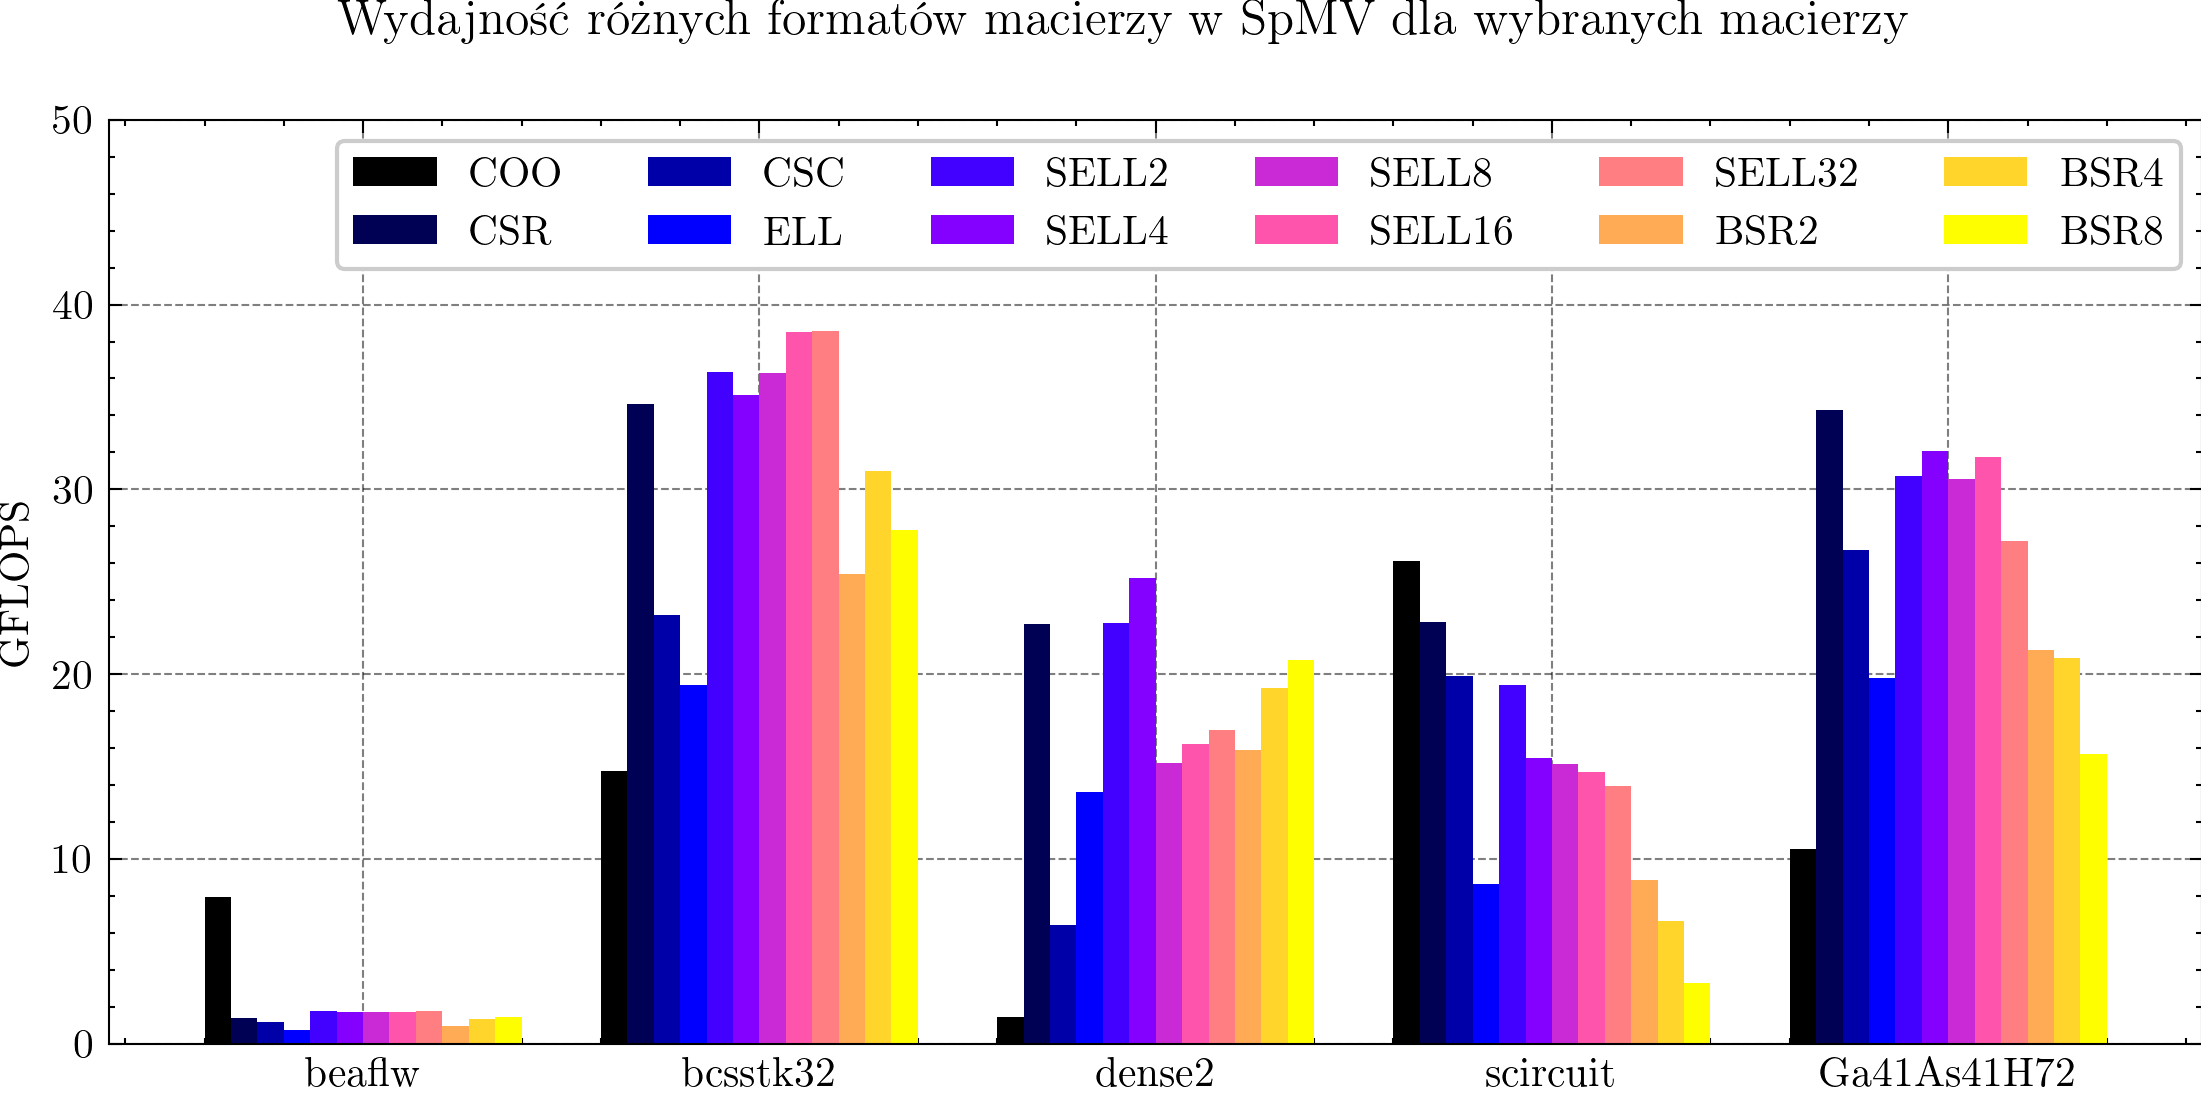
\includegraphics[width=\linewidth]{result_plots/barchart.png}
    \caption{Wydajność różnych formatów macierzy}\label{all_plot}
\end{figure}

Wprowadzono pojęcie efektywności formatu, który jest sposobem porównania efektywności wykorzystania pamięci do uzyskania danego poziomu wydajności obliczeniowej, określonego przez stałą $k$:

\begin{equation}
    k = \frac{1}{t \cdot s}
\end{equation}

\begin{eqwhere}[2cm]
	\item[$k$] stała efektywności
	\item[$t$] czas obliczeń
    \item[$s$] rozmiar pamięci potrzebny do reprezentacji macierzy
\end{eqwhere}

Pozwala ona na porównanie w kontekście tej samej macierzy wydajności obliczeniowej w zależności od ilości wykorzystanej pamięci.
Stała ta faworyzuje jak najmniejsze wykorzystanie pamięci i w tym samym momencie jak najszybsze wykonanie programu, format może wykorzystać więcej pamięci, jeżeli czas wykonania na tym drastycznie zyskuje.
Porównywanie różnych stałych może zostać dokonane tylko w obrębie tej samej macierzy.
Celem ułatwienia porównań na wykresie \ref{all_k_plot} przedstawiono każdą wartość $k$ przeskalowaną względem stałej $k$ dla formatu CSR.
W skutek tego w każdej macierzy format CSR zyskuje wartość $k = 1$, pozostałe wartości należy interpretować jako mnożnik efektywności tego formatu dla tej macierzy względem formatu CSR.
Wybrano CSR ze względu na średnio najwyższe wyniki oraz stosunkowo niskie zużycie pamięci.
W dwóch przypadkach macierzy, format CSR jest najbardziej efektywnym formatem, dla macierzy \textit{DENSE2} jest prawie dwa razy mniej efektywny niż BSR dla rozmiaru bloku równego $8$, dla macierzy \textit{BEAFLW} jest drugi co do efektywności względem formatu COO, która jest 2.5 raza bardziej efektywna i dla BCSSTK32 jest prawie na równi z wariantami SELL i BSR.

\begin{figure}[!htb]
    \centering
    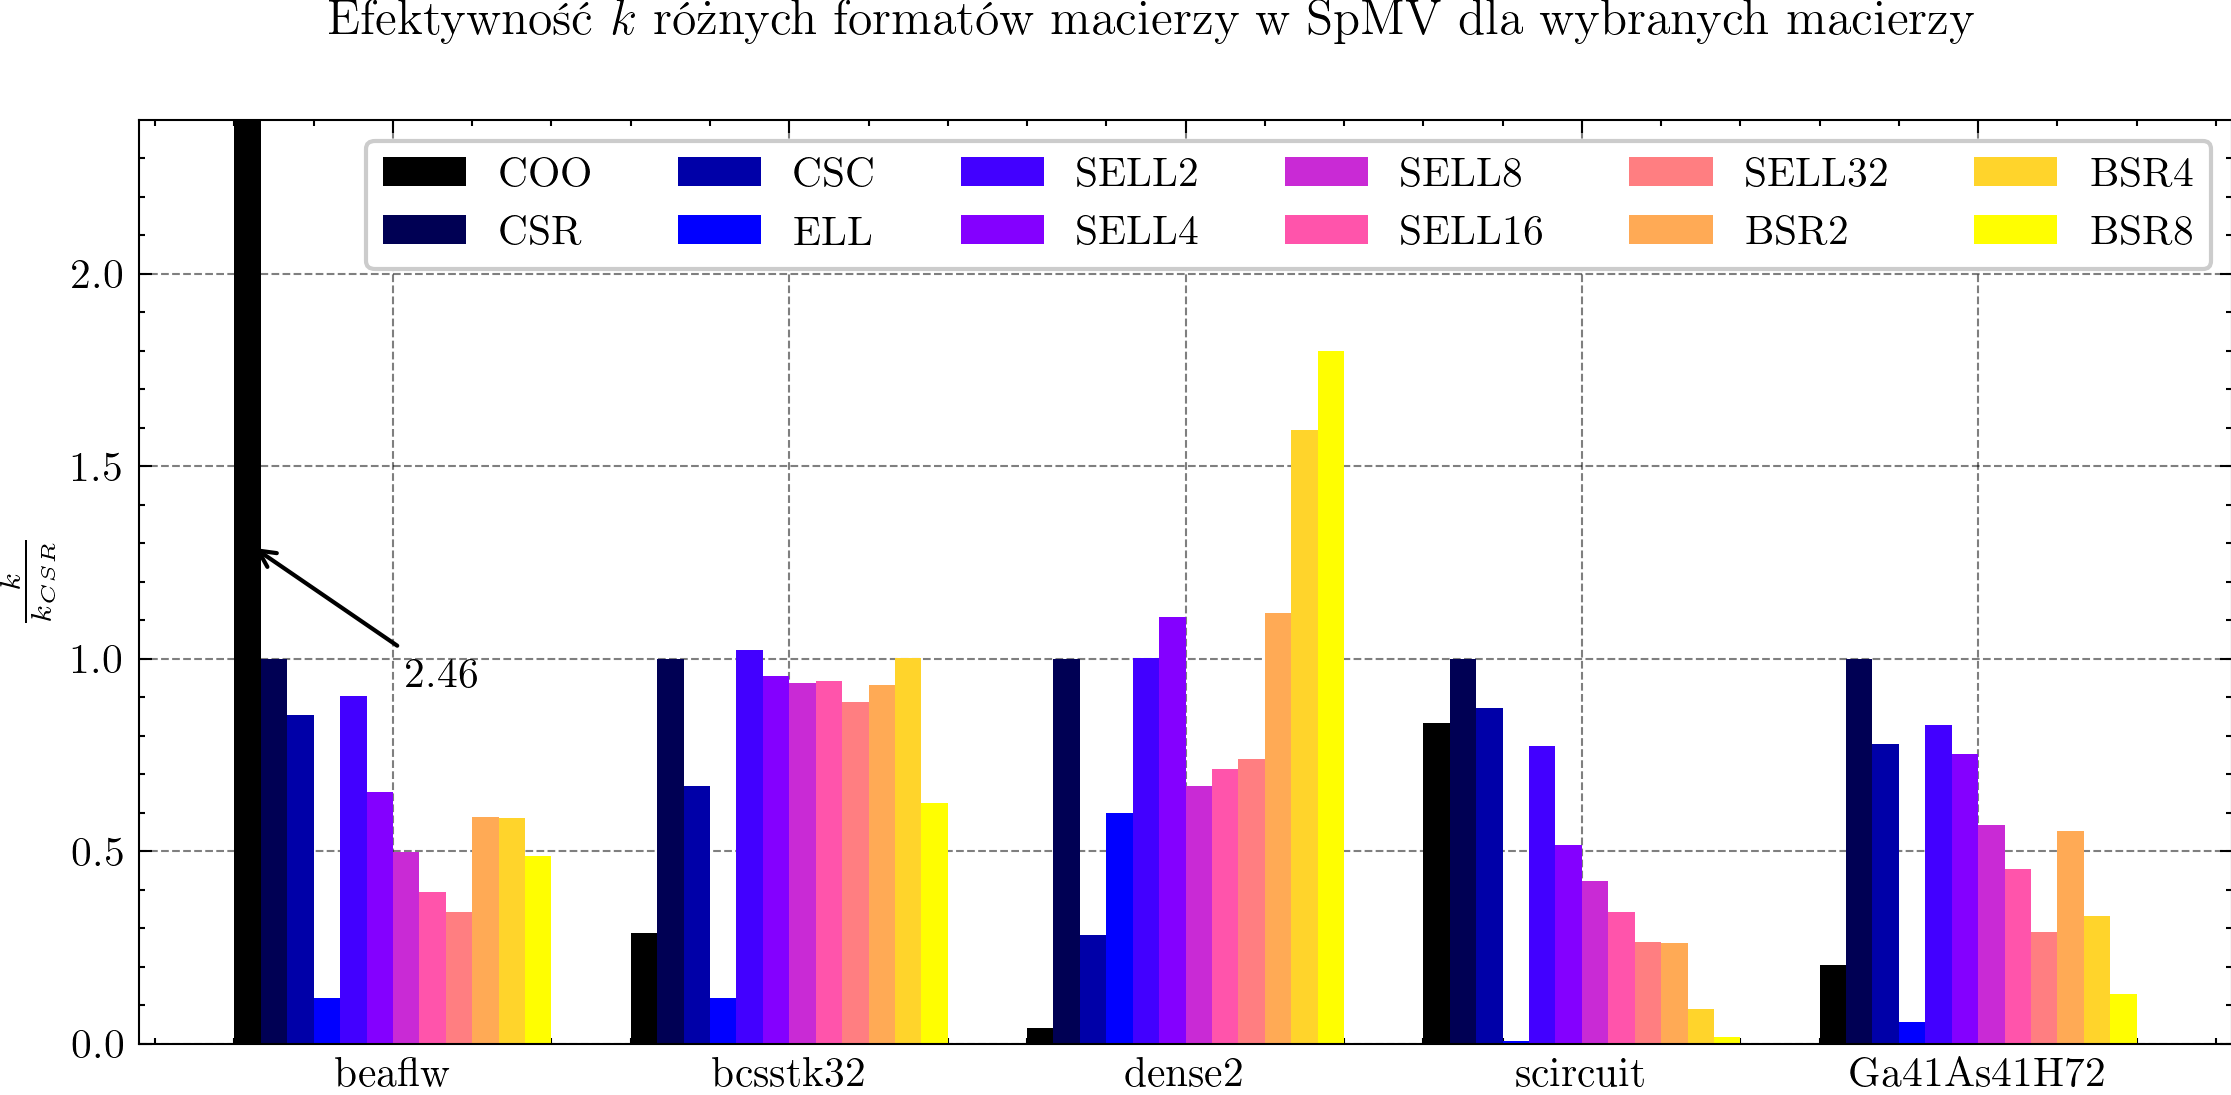
\includegraphics[width=\linewidth]{result_plots/barchart_memory.png}
    \caption{Porównanie efektywności wykorzystania pamięci}\label{all_k_plot}
\end{figure}

Finalne wyniki posiadały pewne różnice pomiędzy sobą, największy błąd względny pojedynczego elementu wektora wyjściowego, dla którego bazą był wynik obliczony na jednostce centralnej formatem ELL wynosił $1.894\%$ dla formatu CSC w macierzy GA41AS41H72.
Różnice te są oczekiwanym rezultatem zmiany kolejności wykonywania obliczeń, ponieważ standard IEEE-754  \cite{FloatPoint} nie gwarantuje łączności obliczeń.
Przez to należy rozumieć, iż zachodzi następująca nierówność:

\begin{equation}
    (x+y)+z \neq x+(y+z)
\end{equation}

Połączenie formatu, który rozdziela pracę w przeciwnym kierunku co format ELL oraz atomicznej redukcji do każdego elementu wektora wyjściowego, tworzy środowisko, w którym oczekiwane będzie, iż kolejność wykonywanych operacji będzie różna od tej, która miała miejsce podczas obliczeń na jednostce centralnej.
Dodatkowo, duża ilość elementów i niejednolite wartości macierzy GA41AS41H72 tylko potęgują ten efekt.

Obliczenia wymagane do wykonania operacji iloczynu macierz-wektor są proste, jedno mnożenie i jedno dodawanie dla każdego elementu macierzy, dlatego tego mikroprocesor przez większość czasu zawsze będzie czekać na pamięć potrzebną do wykonania zadanych operacji.
Mierzony czas w większości algorytmów będzie jedynie czasem potrzebnym na załadowanie danej macierzy z pamięci głównej operacyjnej procesora graficznego do jego rejestrów.
Przez to czynnikiem limitującym teoretyczne maksimum wydajności będzie maksymalna przepustowość pamięci głównej.
Na wykresie \ref{absolute_tput} ukazano całkowitą przepustowość jako ilość pamięci potrzebnej do reprezentacji danej macierzy podzieloną przez średni czas wykonania algorytmu.
Aby określić maksymalną przepustowość pamięci procesora graficznego należy znać taktowanie pamięci, szerokość szyny pamięci i typ pamięci, który jest zainstalowany ze względu na fakt, iż różne typy mogą dostarczyć więcej niż jeden bit danych w każdym cyklu.
Używając następującego równania:

\begin{equation}
    T = G f_m (w_b / 8)
\end{equation}

\begin{eqwhere}[2cm]
	\item[$T$] teoretyczna maksymalna przepustowość pamięci
    \item[$G$] ilość bitów przesyłanych w każdym cyklu przez pamięć 
	\item[$f_m$] taktowanie pamięci
    \item[$w_b$] szerokość szyny w bitach
\end{eqwhere}

Na podstawie tego równania określono maksymalną przepustowość pamięci na wartość równą 336GB/s, algorytmy zbliżające się do tej wartości można uznać za optymalne, ponieważ wykorzystują całą dostarczoną im pamięć bezstratnie.
W budowaniu wykresu pomięto format ELL, gdyż ciężko jest określić jaka część pamięci została załadowana ze względu na fakt, iż obliczenia mogą zostać zakończone, jeżeli dane w danym rzędzie się skończyły.

\begin{figure}[!htb]
    \centering
    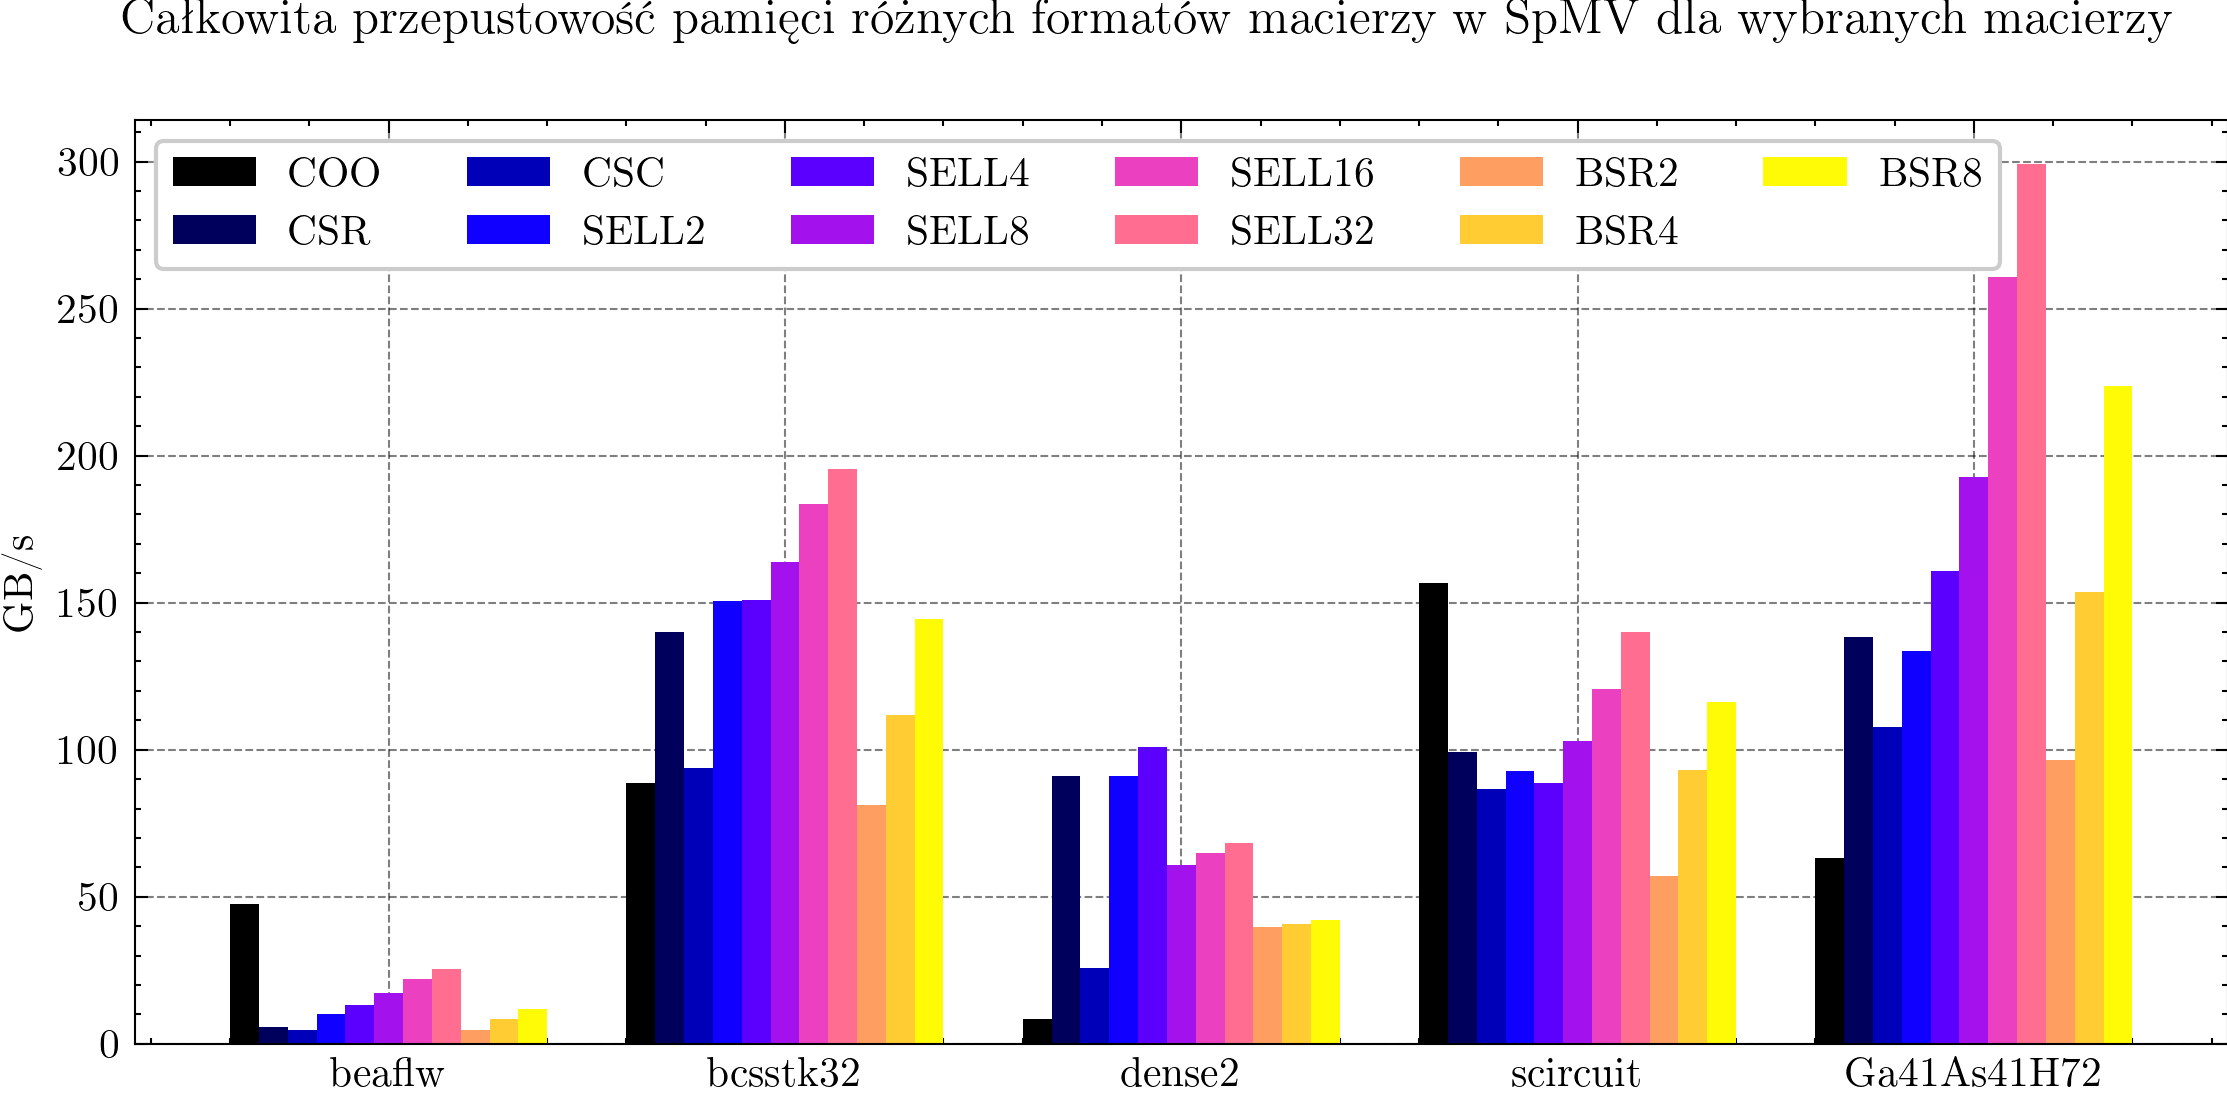
\includegraphics[width=\linewidth]{result_plots/barchart_memory_absolute_tput.png}
    \caption{Porównanie całkowitej przepustowości pamięci}\label{absolute_tput}
\end{figure}

Na wykresie można zauważyć, że formatem najbliżej teoretycznego limitu jest SELL, gdy $C = 32$ dla macierzy Ga41As41H72, ten rozmiar paska równy jest rozmiarowi \textit{warp}'u dla procesorów graficznych NVIDIA.
Wzrost przepustowości wraz ze wzrostem $C$ dla formatu SELL, można wytłumaczyć łączeniem dostępu do pamięci pomiędzy wątkami wewnątrz pojedynczego \textit{warp}'u.
Jeżeli wszystkie wątki wykonują wczytywanie z kolejno po sobie występującej pamięci, kontroler może połączyć wszystkie zapytania w jedno, co zmniejsza narzut na szynę pamięci procesora graficznego.
W prawie każdym przypadku CSR posiada drugą najwyższą przepustowość pamięci po SELL, nie przekracza ona natomiast nigdy progu $50\%$, co wskazuje na pole do optymalizacji, którą udało się osiągnąć w praktyce\cite{AMD_CSR_opt}.
Format COO i CSC wykazują w większości najniższe przepustowości, najprawdopodobniej ze względu na kolizję w operacjach atomicznych.
BSR wykazuje niską przepustowość całkowitą na pewnych macierzach natomiast wysoką na innych, format ten jest dobrym kandydatem na głębszą analizę wydajnościową przy wykorzystaniu takich narzędzi jak NVIDIA NSight.

NVIDIA NSight to zestaw narzędzi pozwalających na pracowanie z programami graficznymi, gdy uruchomione one zostaną na procesorze graficznym firmy NVIDIA.
Dla \textit{Vulkan} istnieje możliwość zebrania danych na temat wykorzystania procesora graficznego przy użyciu \textit{NSight Graphics}\cite{nsight}, używając opcji \textit{GPU Trace}, ten pozwoli nam zebrać takie dane jak te w ilustracji \ref{nsight_results}.
Są to między innymi metryki odnośnie przepustowości pamięci w każdej z pamięci podręcznych, nietrafienia w pamięć podręczną, wykorzystanie rejestrów i wiele innych.
Na ich podstawie możliwe jest dokonanie decyzji, które poprawi dany aspekt rozwiązania w taki sposób, aby rzecz będąca czynnikiem limitującym była zminimalizowana w najbardziej możliwy sposób.

\begin{figure}[t]
    \centering
    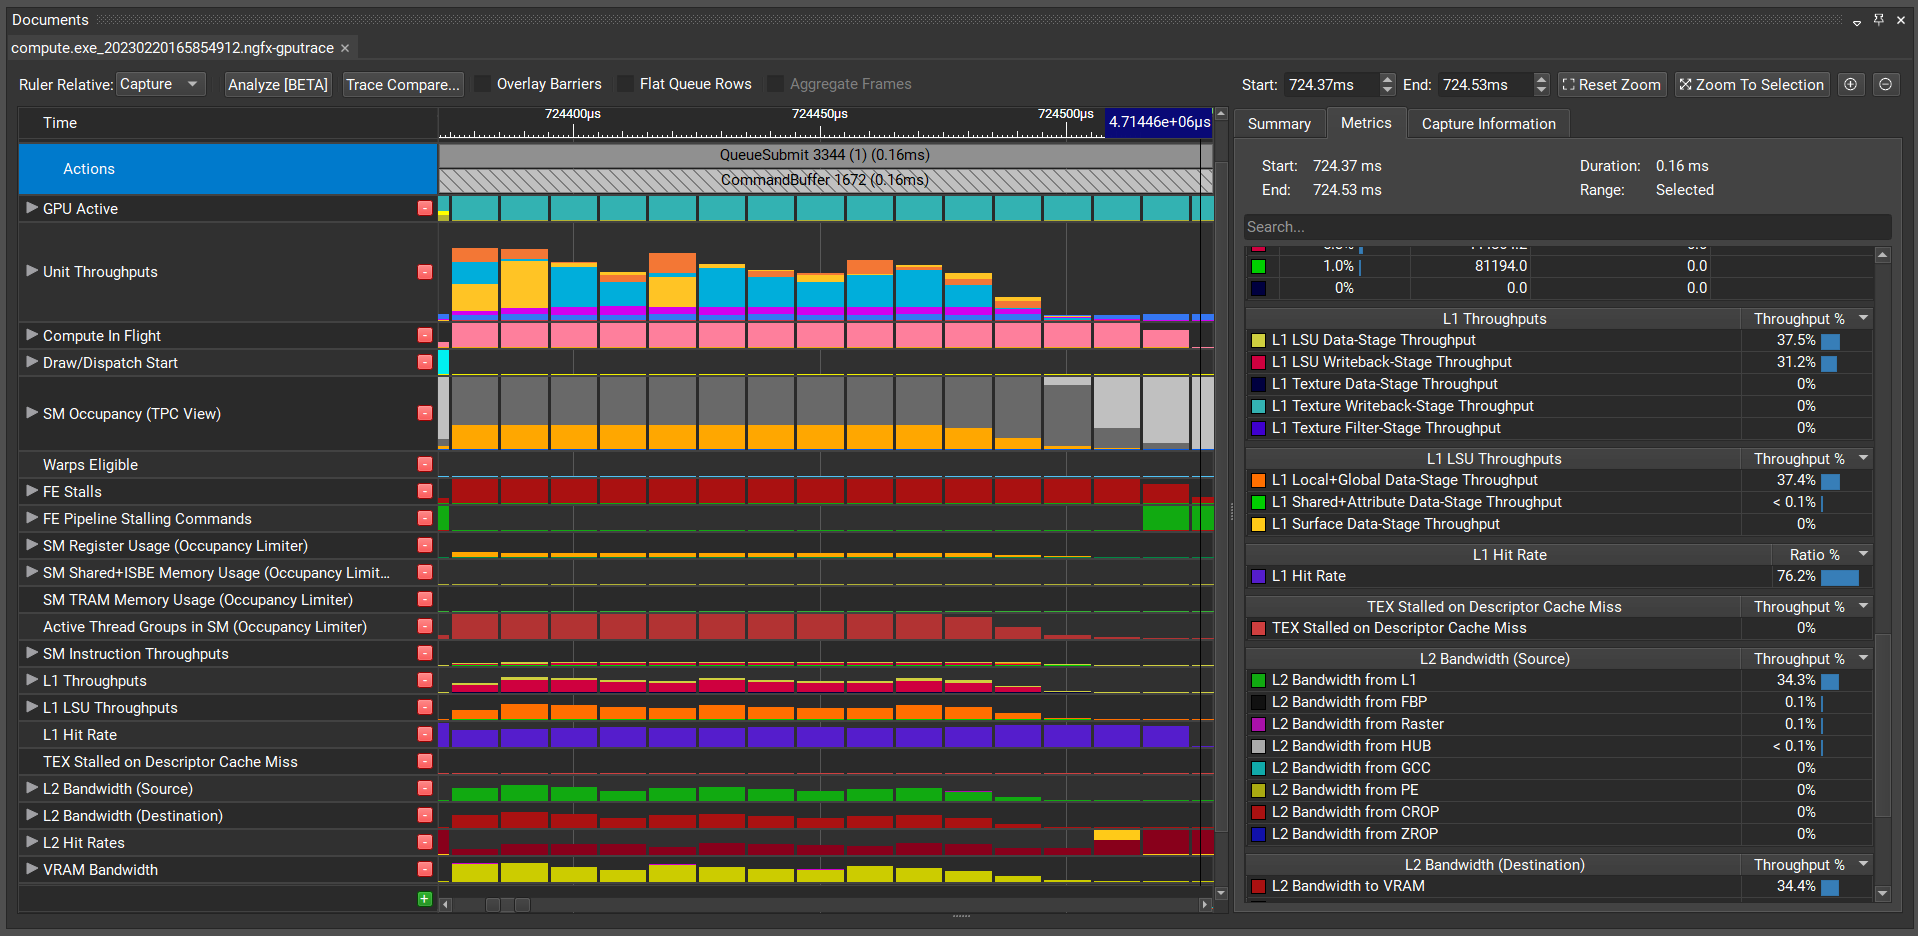
\includegraphics[width=\linewidth]{misc_figs/nsightgraphics.png}
    \caption{Metryki zebrane z uruchomienia shadera w NSight Graphics}\label{nsight_results}
\end{figure}